\documentclass[10pt, a4paper]{article}

\usepackage[paper=a4paper, left=1.5cm, right=1.5cm, bottom=1.5cm, top=3.5cm]{geometry}
\usepackage[utf8]{inputenc}
\usepackage[spanish]{babel}
\usepackage{graphicx}
\usepackage{multicol}
\usepackage[usenames,dvipsnames]{color}
\usepackage{amsmath}
\usepackage{verbatim}
\usepackage{footnote}
\usepackage{float}
\usepackage{amsfonts}
\usepackage{hyperref}
\usepackage{framed}
\usepackage{pdflscape}

\usepackage{pdfpages}

\usepackage{caratula}


\materia{Ingeniería de Software II}

\titulo{Trabajo Práctico 1}
\subtitulo{Sprint Planning}

\integrante{Mart\'in Alejandro Miguel}{181/09}{m2.march@gmail.com}
\integrante{Ivan Postolski}{216/09}{ivan.postolski@gmail.com}
\integrante{Juan Manuel Martinez Camaño}{276/09}{jmartinezcaamao@gmail.com}
\integrante{Matias Incem}{396/09}{matias.incem@gmail.com}
\integrante{Pablo Gauna}{}{}

\begin{document}

\maketitle
\tableofcontents
\newpage

	\section{Product backlog}
		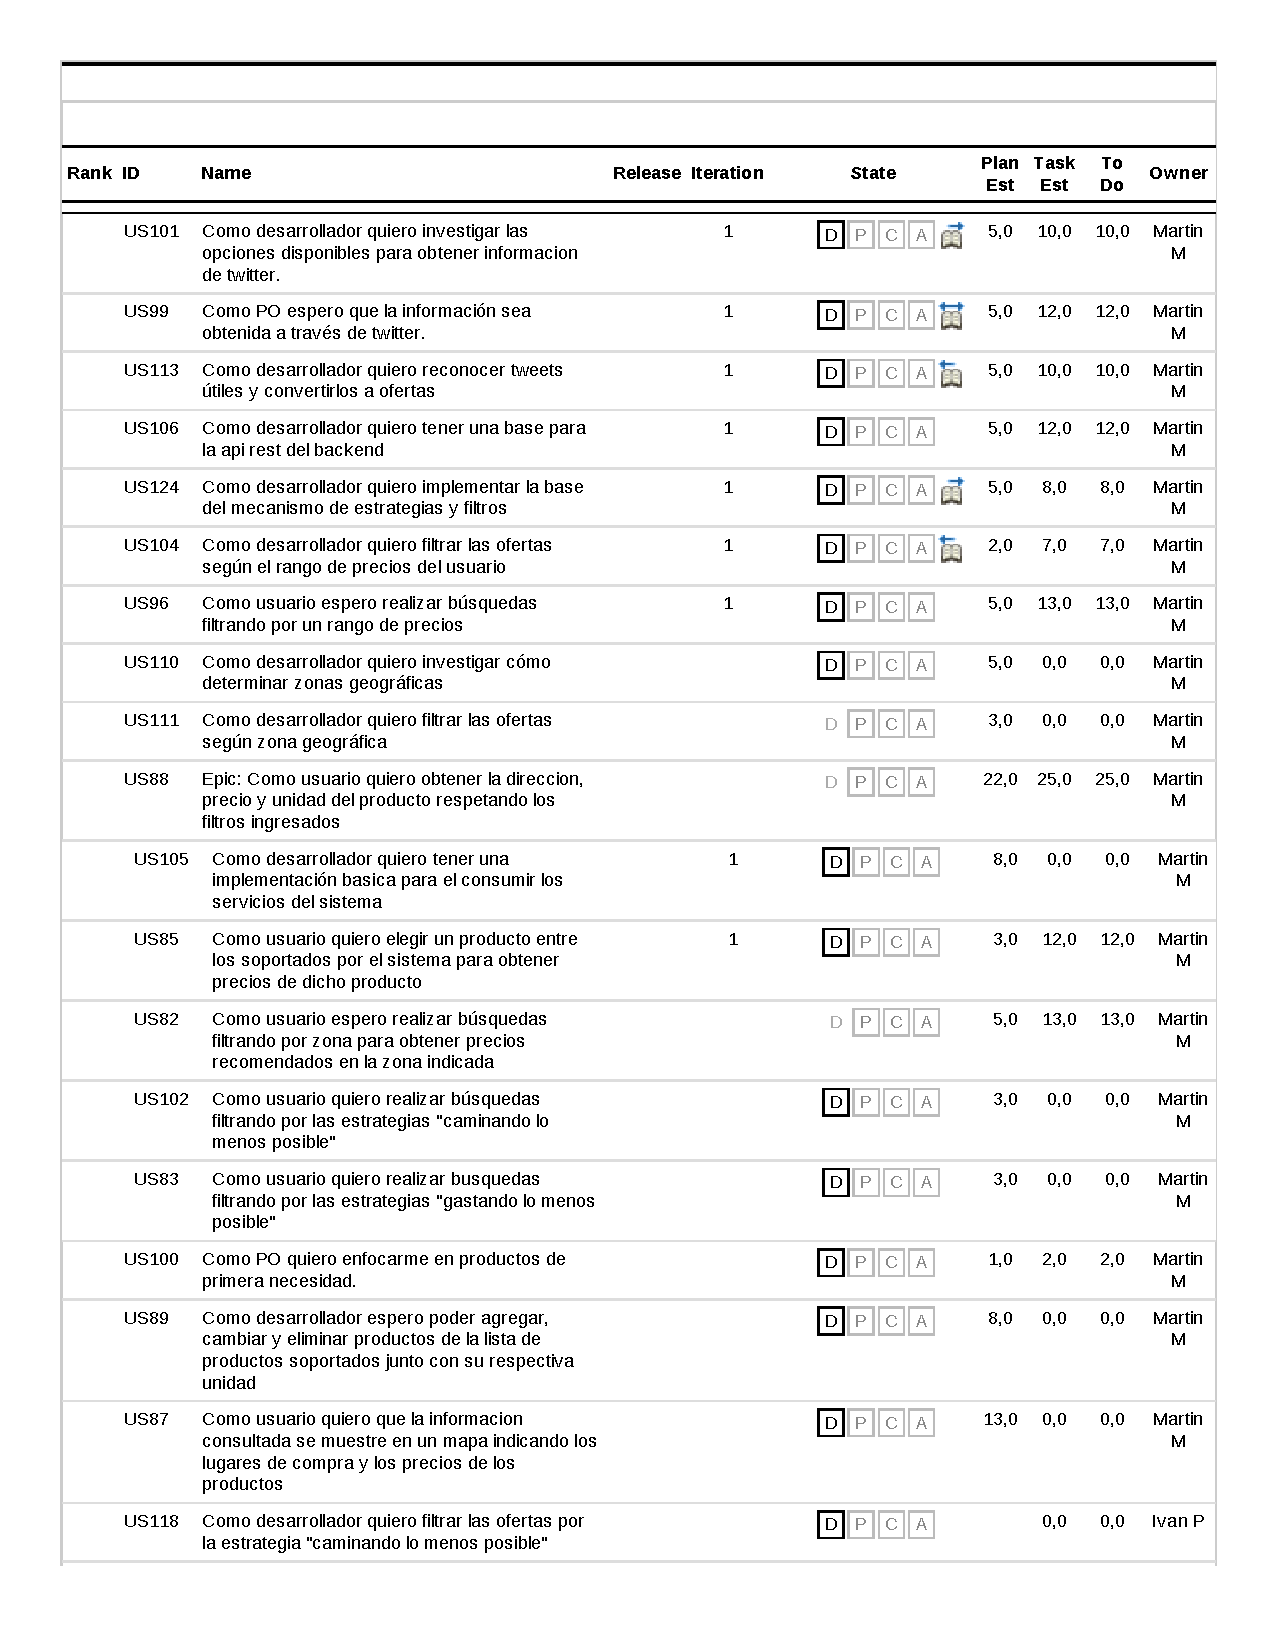
\includepdf[pages={1,2}]{product_backlog.pdf}

	\section{Sprint backlog}
		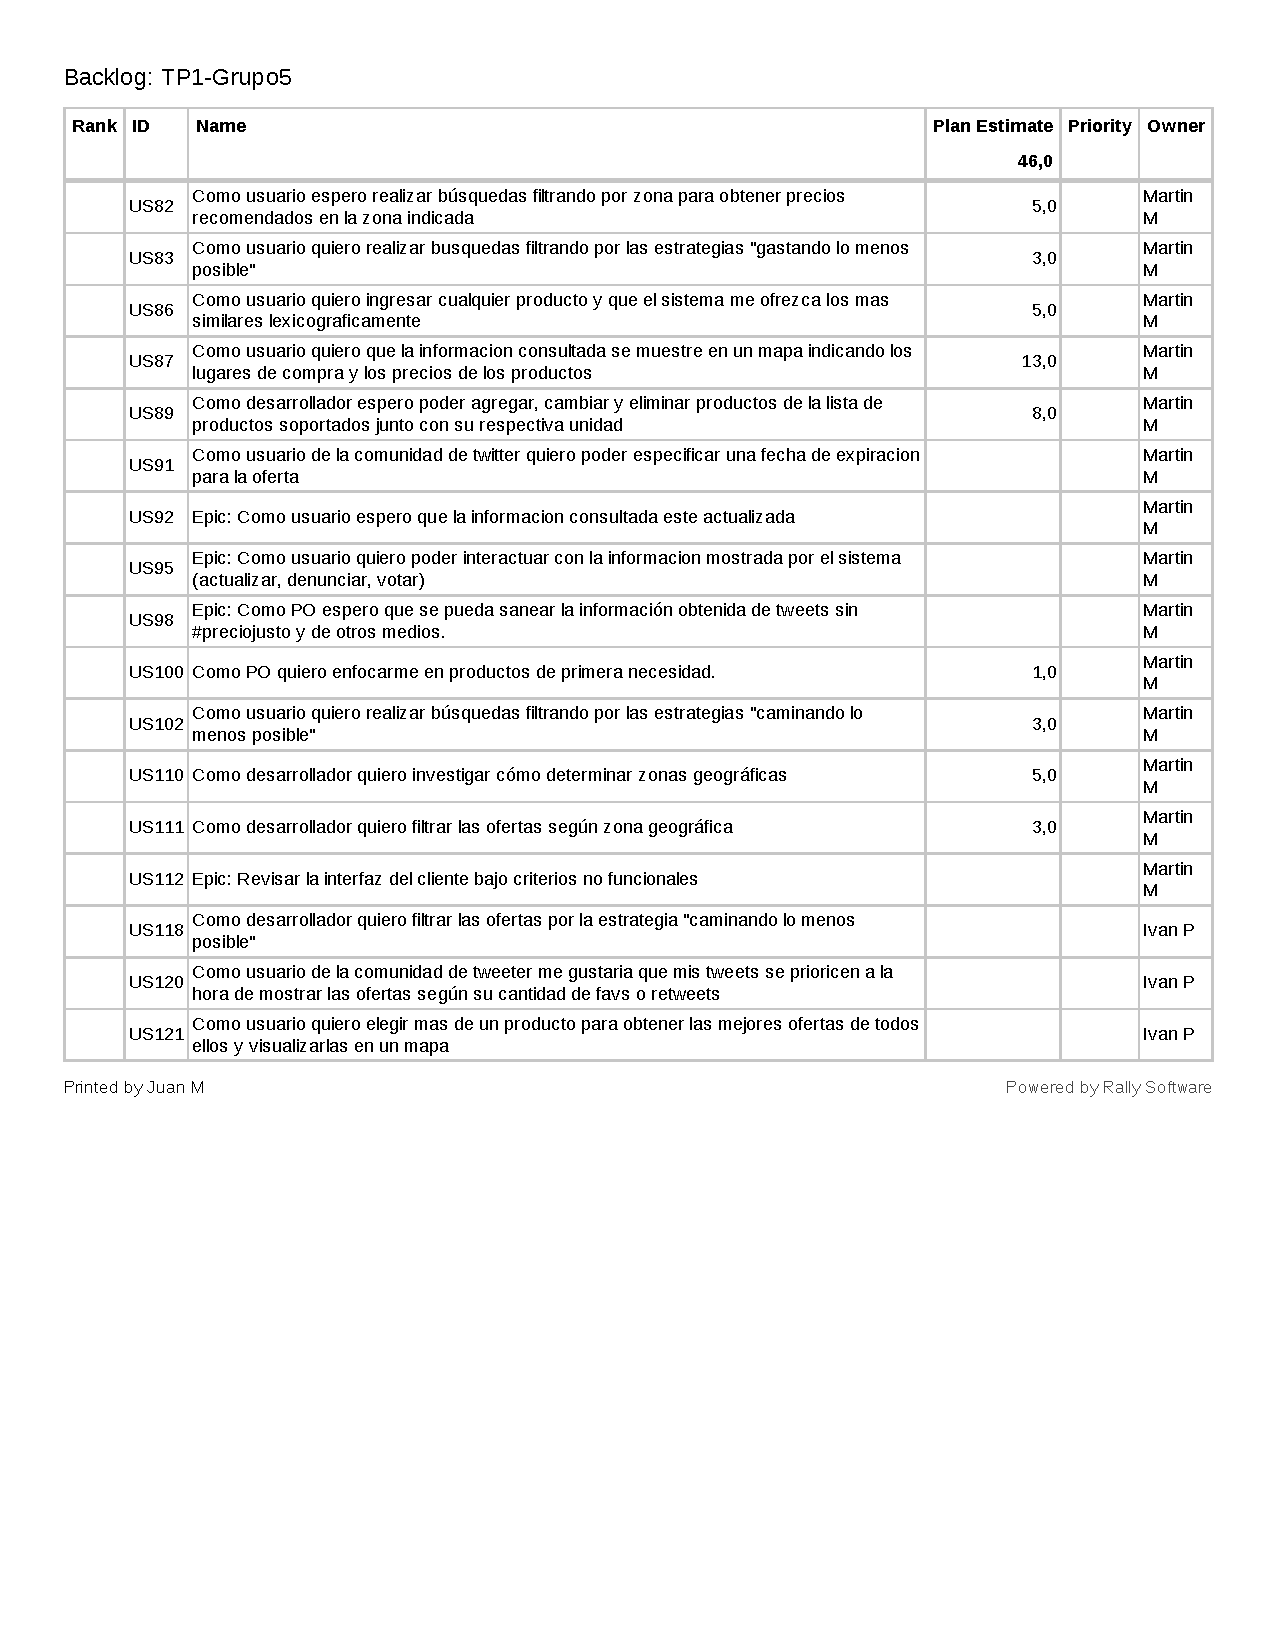
\includepdf[pages={1}]{sprint_backlog.pdf}

  \begin{landscape}
  \section{Análisis del sistema}
  \begin{figure}[H]
      \centering
      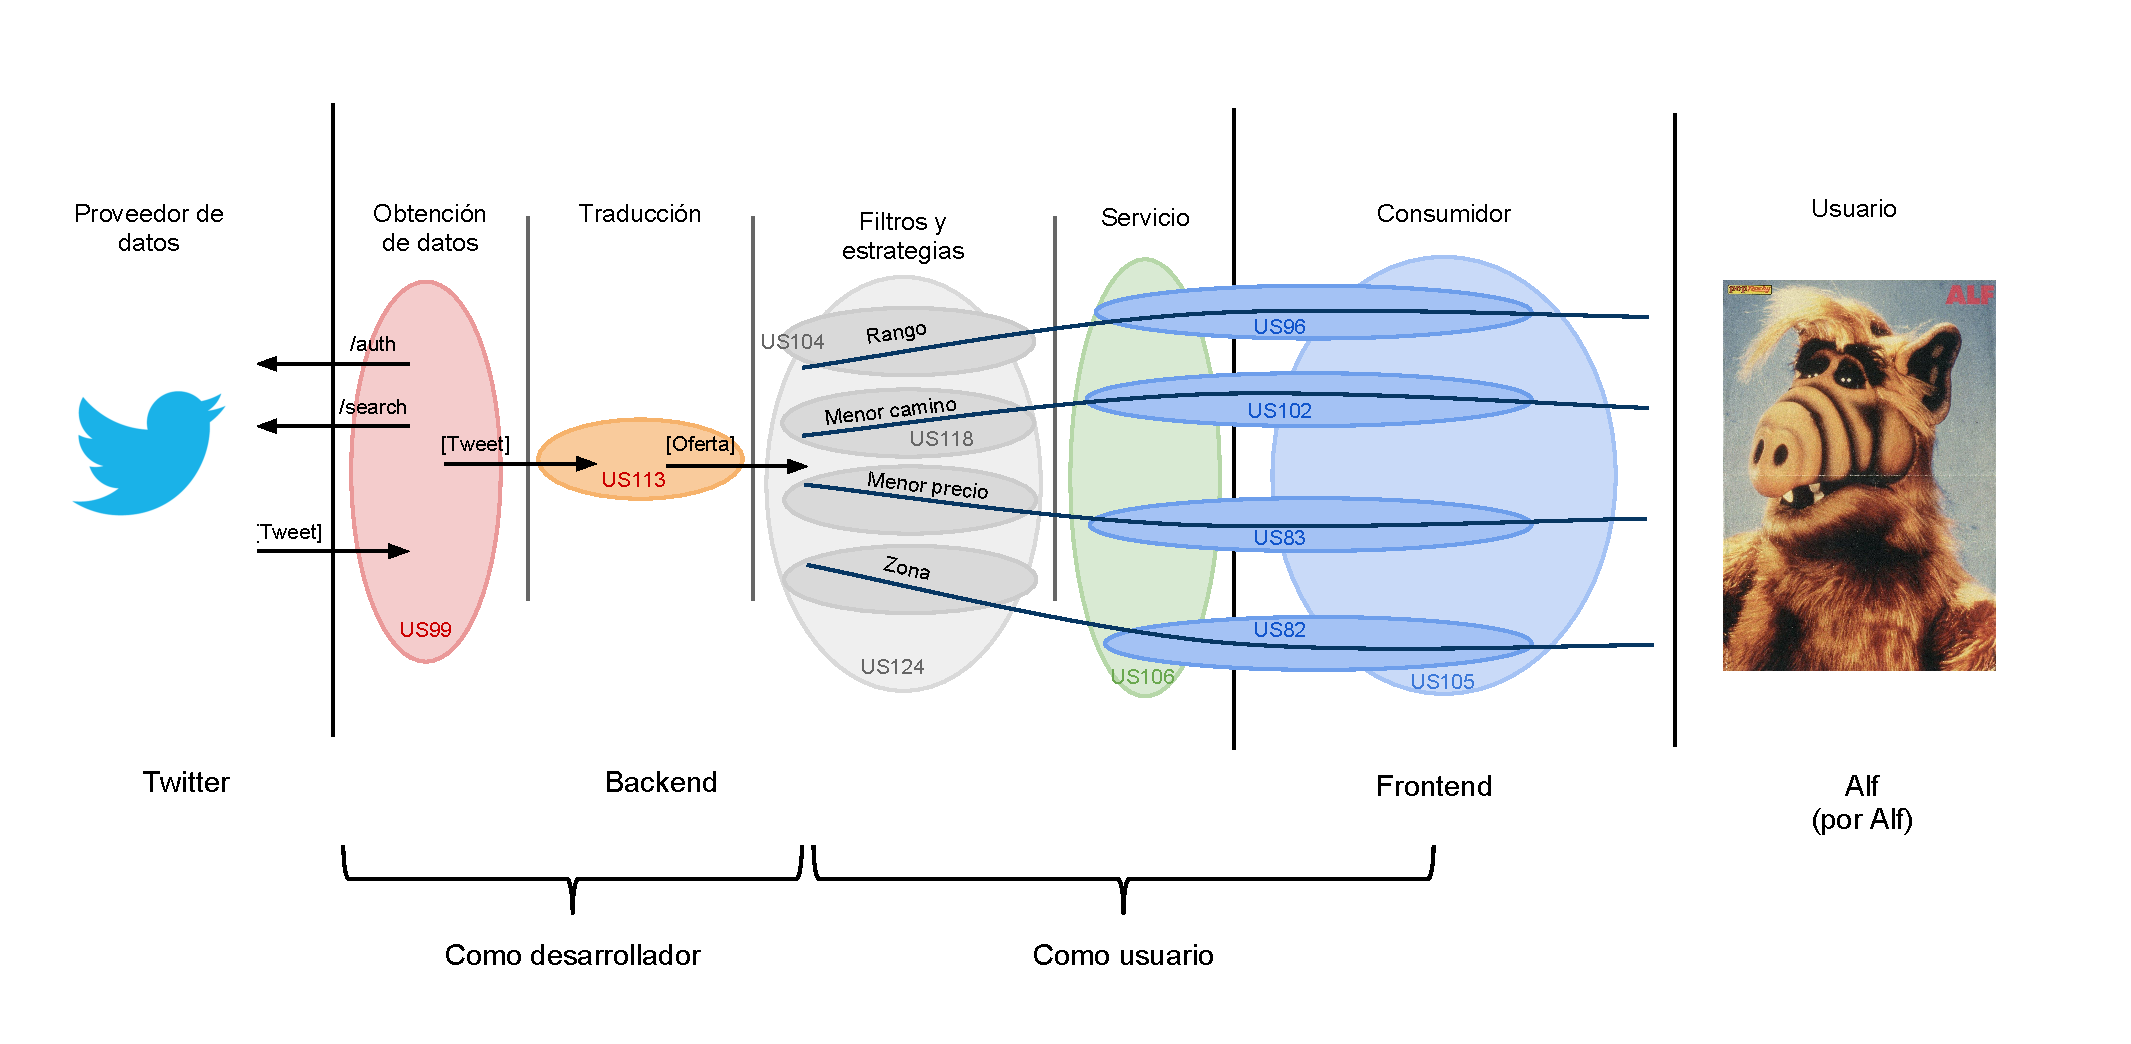
\includegraphics[scale=0.8]{graphics/arch_diagram.pdf}
      \caption{Diagrama de arquitectura (primer boceto)}
    \end{figure}
  \end{landscape}

  El diagrama presentado anteriormente es una aproximación informal de la arquitectura del sistema, que sirve para entender la estructura 
  de las \textsf{User Stories} definidas respecto a la primera concepción del mismo. Cada círculo consituye una \textsf{User Story} (aunque no todas las
  \textsf{User Stories} se encuentran en el diagrama). Cuando un círculo se encuentra por debajo de otros es porque esta \textsf{User Story} es predecesora
  de las otras (i.e. debe realizarse antes).


  \subsection{Definiciones}
  \begin{itemize}
    \item\textbf{Oferta:} Una oferta es la información extraída de un tweet que cumple con el formato del \emph{Precio Justo}.
    Una oferta posee un producto, un precio por una cierta unidad y una ubicación. En una primera instancia la ubicación sería
    un texto indicando calle y altura, en un futuro esta podría ser un punto geográfico representado ya validado por el sistema
    (por ejemplo, si se incluye la información de georeferenciación de twitter). Las \textsf{ofertas} será lo que finalmente se
    muestra al usuario.

  \item\textbf{Filtro:} Un filtro de ofertas define si una Oferta cumple con un criterio para luego descartarlo de los
    resultados en caso de no cumplirlo.

  \item\textbf{Estrategia:} Una estrategia separa un subconjunto de \textsf{Ofertas} utilizando información global de los mismos
    (por ejemplo al buscar menor precio busca los mínimos del conjunto segun el precio de cada oferta).
  \end{itemize}

  \subsection{Criterios}
  \begin{itemize}
    \item\textbf{Cantidad de productos:} en una primera instancia la aplicación estará trabajando con consultas para un único producto por vez, 
      dejando la complejidad de utilizar varios para próximas iteraciones.
    \item\textbf{Responsabilidad de la información:} durante el debate de definición de la aplicación surgió el problema de cómo hacer que los datos
      provistos por la aplicación sean correctos o, en todo caso, a quién le corresponde esta responsabilidad. Una primera forma de ver la aplicación
      fue como alguién que recorre twitter y reproduce la información del mismo de forma ordenada y sin ruido. En este caso, la aplicación se separa
      de la responsabilidad de que la información mostrada sea correcta. No obstante, surgieron ideas respecto a como tener mayor seguridad sobre la 
      ofertas exhibidas. Una primera aproximación fue utilizar siempre la oferta más nueva para un producto en un lugar, considerando que si dos tweets
      hablan de lo mismo el más nuevo tiene datos más actualizados. Otra idea fue no mostrar información que fuese más antigua que cierto tiempo, 
      denominado \texttt{freshness}. Finalmente se planteó que nuestro sistema podría actuar como una base de datos de información de precios en negocios
      que se actualiza desde distintas fuentes. Así existiría una alta, baja y modificación de ofertas, donde incluso los mismos usuarios de la aplicación
      podrían contribuir a la misma sin utilizar twitter. Esta última opción hace al sistema completamente responsable de los datos provistos al usuario.
    \item\textbf{Ofertas de tiempo limitado:} relacionado con el concepto de \texttt{freshness} surgió la idea de que podrían existir ofertas de tiempo 
      limitado (como ser "kilo de naranjas \$4 este fin de semana"). Es de interés considerar en un futuro la posibilidad de que los usuarios puedan
      reportar este tipo de ofertas con toda su información. Mientras tanto, se decidió considerar que \emph{todas} las \textsf{ofertas} tendrán un
      tiempo de expiración por defecto (lo cual también es útil para mantener la información correcta).
  \end{itemize}


\end{document}
